\chapter{Algorithmen}\label{ch:algorithmen}
Forschungsfrage überlegen (Warum nicht DB zum Speichern von Spielerdaten)

Verschiedene Theorien von Speicher und Ladesysteme ausarbeiten und Zeiten 
messen (Mit Java und JSON erst mal). Verschiedene Spielarten und Speichersysteme
für diese ausarbeiten (Chunk Systeme machen vielleicht nicht überall Sinn, aber 
allgemein Daten aufteilen müsste gut sein)
%--------------------------------------------------------------------------
%--------------------------------------------------------------------------





%--------------------------------------------------------------------------
%--------------------------------------------------------------------------
\section{Speichersysteme}\label{sect:speichersysteme}
Erstmal Theorie von Speichersystemen und Bezug auf Arten von Videospiel-Daten.

Theorie durch Daten/einfaches Spielkonzept mit Java und JSON testen:\\
-Spieler (HP, LVL, Ausrüstung, Position, Rotation, ...)\\
-Gegner (HP, LVL, Ausrüstung, Position, Rotation, ...)\\
-Ausrüstung (Beschreibung/ID, Verteidigung, Angriff)\\
-Hindernisse (Beschreibung/ID, Position, Rotation)\\
-Items (Beschreibung/ID, Position, Rotation)\\
-> Klassendiagramm zeigen, um Daten des Spieles zu visualisieren

Wichtiger unterschied zwischen ersten Speichern und das Speichern Danach
(beim ersten Mal muss die Grundstruktur aufgebaut werden und die random
erstellte Map gespeichert werden)
%--------------------------------------------------------------------------


%--------------------------------------------------------------------------
\subsection{Daten in Videospielen}
Statische Daten (Maps, Texturen, etc.) und sich ändernde Daten (Spielerdaten und 
Daten zu dem Spielstand). Fokus dieser Arbeit sind nicht die statischen Daten!

Typen von Daten:\\
\begin{itemize}
    \item Statische Daten
    \begin{itemize}
        \item Grafikdaten
        \item Audiotechnische Daten
        \item Level- oder Kartendaten
    \end{itemize}
    \item Dynamische Daten
    \begin{itemize}
        \item Spielstand
        \item Benutzerdaten
    \end{itemize}
\end{itemize}
%--------------------------------------------------------------------------


%--------------------------------------------------------------------------
\subsection{Spielphasen}
Verschiedene Phasen ansprechen, die interessant für's Speichern und Laden sind.\\
1. Neues Spiel laden oder altes Spiel laden\\
2. Events in Spiel (Spieler bewegt sich, Item spawned, ...) -> Events speichern\\
3. Chunk Laden 

\begin{figure}[H]
    \centering
    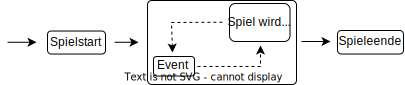
\includegraphics[scale=0.5]{images/Spielphasen.png}
    \caption{Phasen eines Spieles}
    \label{fig:spielphasen}
\end{figure}


Event = Spielobjekt hat sich verändert oder wurde hinzugefügt/gelöscht.
%--------------------------------------------------------------------------


%--------------------------------------------------------------------------
\subsection{Delta basierte Speicherung}
Das wichtigste um die Menge der gespeicherten Daten zu reduzieren, ist, dass man nur nur veränderte Daten speichert. 
\begin{itemize}
    \item Neue Elementen
    \item Elemente verändern sich
    \item Elemente werden gelöscht
\end{itemize}
Gespeicherte Daten müssen diese drei Veränderungen berücksichtigen
%--------------------------------------------------------------------------


%--------------------------------------------------------------------------
\subsection{Aufteilung der Daten}
Chunking\\
\begin{itemize}
    \item Aufteilung der Mengen an Daten unter den Chunks
    \item Datengröße kann sich stark verändern, Chunk System muss sich anpassen
    \item Wenn Daten zu viele werden mehr Chunks
    \item Wenn Daten zu wenig werden weniger Chunks
    \item Chunk System nach Area, damit Laden effizienter läuft 
    (Nur Chunks mit seinen Elementen laden, wenn dieser in Nähe ist)
\end{itemize}

Sharding (Mehr was für Kapitel Datenbanken)
%--------------------------------------------------------------------------


%--------------------------------------------------------------------------
\subsection{Komprimierung der Daten}
Zippen der Daten\\
\begin{itemize}
    \item Viel zippen vs. kleine Dateien (Kleine Chunks)
    \item Bringt lokales Zippen überhaupt was oder nur wenn man mit Server arbeitet?
\end{itemize}

Kürzere property Namen\\
Null Werte ausschließen\\
Sowas wie Vectoren (x,y,z,...) als ein String speichern?
%--------------------------------------------------------------------------


%--------------------------------------------------------------------------
\subsection{Kodierung der Daten}
Eigentlich auch eine Art der Komprimierung der Daten, wenn richtig gemacht.\\
JSONH zum Beispiel (\url{https://stackoverflow.com/questions/11160941/is-it-worth-the-effort-to-try-to-reduce-json-size})

Binäre Serialisierung?

\subsection{Serialisieren}
Effizientes schreiben in (JSON) Datenbanken.\\\\
Arten um mit JSON zu arbeiten:
\begin{itemize}
    \item Streaming API
    \item Tree Model
    \item Data Binding
\end{itemize}
(Siehe \url{https://www.tutorialspoint.com/jackson/jackson_overview.htm})
%--------------------------------------------------------------------------


%--------------------------------------------------------------------------
\subsection{Schreibprozesse reduzieren}
Das Schreiben in den normalen Speicher ist zeitintensiv. Deshalb sollte möglichst wenig Daten auf die Festplatte geschrieben werden. Eine Möglichkeit ist es, die veränderungen über eine Liste im Arbeitsspeicher zu speichern und bei Programmterminierung diese Liste abzuspeichern. Dies ist aber riskant, da Daten verloren gegangen werden können bei frühzeitigen Löschen. Alternativ kann man diese Liste auf dem Festplattenspeicher führen und beim Laden des Spieles abarbeiten und dann leeren.

%--------------------------------------------------------------------------


%--------------------------------------------------------------------------
\subsection{Speicherstrategien}
Kurz das kleine Java Projekt vorstellen mit den Beispieldaten die gespeichert und geladen werden sollen. Erwähnen, dass JMH zum messen der Effizienz der Strategien verwendet wurde.\\

Faktoren:\\
\begin{itemize}
    \item Chunk size
    \item Veränderungen
\end{itemize}
%--------------------------------------------------------------------------
%--------------------------------------------------------------------------




%--------------------------------------------------------------------------
%--------------------------------------------------------------------------
\section{Ladesysteme}\label{sect:ladesysteme}
Erstmal Theorie vom Laden der Spieldaten erarbeiten. Danach mit Spielkonzept
von 2.1 testen und Laufzeiten messen.
%--------------------------------------------------------------------------


%--------------------------------------------------------------------------
\subsection{Nearby Loading}
Nur die Daten laden, die in der Nähe vom Spieler sind (über Render-Distance)\\
Chunk System dafür sehr vorteilhaft für effizienteres Laden, statt durch alle Elemente
immer zu iterieren.
%--------------------------------------------------------------------------


%--------------------------------------------------------------------------
\subsection{Lazy Loading}
Weiß nicht, ob das der richtige Begriff dafür ist, aber hier soll über das prozedulare 
Laden der Daten geschrieben werden (nicht alles auf einmal laden, sondern erst mal nur das
nötigste und dann Stück für Stück den Rest laden). 
%--------------------------------------------------------------------------


%--------------------------------------------------------------------------
\subsection{Effizienz der Ladestrategien}
Laufzeiten vom Laden messen. Vielleicht läuft das Laden mit manchen Speicherstrategien 
besser als mit anderen. Außerdem ist die Performance nicht nur an Zeit zu messen, sondern
an Ressourcen, die vom Computer benötigt werden. Vielleicht gibt es Lade Strategien, die
leicht gewichtet laufen können.
%--------------------------------------------------------------------------
%--------------------------------------------------------------------------




%--------------------------------------------------------------------------
%--------------------------------------------------------------------------
\section{Strategien}
Aus den Strategien der vorherigen sections verschiedene Speicherstrategien aufstellen und deren Effizienz auswerten.

Allgemeines Speicher- und Ladesystems (manche Schritte optional)
\begin{figure}[H]
    \centering
    \includegraphics[scale=0.5]{images/Speichersystem.png}
    \caption{Phasen eines allgemeinen Speicher- und Ladesystems}
    \label{fig:speicherphasen}
\end{figure}

\begin{itemize}
    \item Spielstand laden kann alles auf einmal oder nur teile geladen werden (siehe mehr im Kapitel \ref{sect:ladesysteme})
    \item Je nach Speichersystem müssen hier teilweise noch die gespeicherten Daten überarbeitet werden
    \item Je nach Speichersystem können die Events die in "Änderung speichern" behandelt werden in zwei Kategorien unterteilt werden:
    \begin{enumerate}
        \item Ein Spielobjekt wurde hinzugefügt/geändert
        \item Ein Spielobjekt wurde gelöscht
    \end{enumerate}
    \item Spiel laden nach Events, wenn der Spieler sich z.B. in neuen Bereichen der Map befindet, die noch geladen werden müssen (mehr dazu in \ref{sect:ladesysteme})
    \item Spielstand am Ende abspeichern, vor Spielende optional (je nach Speichersystem notwendig)
\end{itemize}

Chunk-basiertes Speichersystem, welches Daten in Chunks verpackt:
\begin{figure}[H]
    \centering
    \includegraphics[scale=0.5]{images/Chunkbasiert.png}
    \caption{Chunk-basiertes System}
    \label{fig:chunkBasedSystem}
\end{figure}

Wobei ein Chunk aus folgenden Variablen besteht:
\begin{figure}[H]
    \centering
    \includegraphics[scale=0.5]{images/Chunk.png}
    \caption{Chunk Klasse}
    \label{fig:chunkClass}
\end{figure}

\begin{itemize}
    \item Chunks haben Position und Größe
    \item Dynamische oder statische Chunk Größe (Entweder alle Chunks feste Größe, oder sie passen sich an Datenmenge an)
    \item Chunks speichern Objekte, die in deren Bereich sind
    \item ParentID und ChildrenIDs sind optional
\end{itemize}

Informationen zu dem System:

\begin{itemize}
    \item Objekte von Chunks in der Nähe des Spielers laden
    \begin{itemize}
        \item Allgemein werden Objekte eines Chunks erst dann laden, wenn es nötig ist (Z.B. Spieler in der Nähe); sowohl am Anfang, als auch während des Spieles
    \end{itemize}
    \item Chunk Veränderungen speichern bei statischer Chunkgröße:
    \begin{itemize}
        \item Daten zu Chunkinhalt komplett neu speichern bei update/added/removed Objekt Event
    \end{itemize}
    \item Chunk Veränderungen speichern bei dynamischer Chunkgröße:
    \begin{itemize}
        \item Daten zu Chunkinhalt komplett neu speichern bei update/added Objekt Event 
        \item Chunkgröße bei added/removed Objekt Event überprüfen
        \item Chunkdaten komplett vom Speicher löschen, wenn dieser im Spiel gelöscht wird (beim Joinen mit benachbarten Chunks)
        \item Chunkdaten updaten und hinzufügen, wenn ein Chunk auf weiter Child-Chunks gesplitted wird
    \end{itemize}
\end{itemize}

Alternative des Chunk-basierten Systems, um weniger Schreibprozesse auf dem lokalen Speicher zu haben:

\begin{figure}[H]
    \centering
    \includegraphics[scale=0.5]{images/Chunkbasiert2.png}
    \caption{Alternative zu dem Chunk-basierten System}
    \label{fig:altchunkBasedSystem}
\end{figure}

\begin{figure}[H]
    \centering
    \includegraphics[scale=0.5]{images/Changes.png}
    \caption{Speichern von Veränderungen}
    \label{fig:changesClass}
\end{figure}

\begin{itemize}
    \item Veränderungen anwenden:
    \begin{itemize}
        \item Liste von Veränderungen des letzten Spielstandes werden lokal gespeichert (zum Beispiel als Objekte wie \ref{fig:changesClass} in JSON)
        \item Verschiedene Events = Unterschiedlich was Object ist
        \item Liste von oben nach unten abarbeiten, da erste Einträge die ältesten sind 
        \item Objekte aus Liste zu Chunk hinzufügen/updaten oder (bei dynamischer Chunkgröße) Chunks die nicht mehr gebraucht werden löschen
        \item Liste leeren
    \end{itemize}
    \item Nearby loading von Chunks wie beim anderen Chunk-basierten System
    \item Chunk-Veränderung speichern:
    \begin{itemize}
        \item Hinzugefügte/Veränderte/Gelöschte Objekte in Change Liste (im Arbeitsspeicher) speichern
        \item Entweder direkt in lokaler Change List Datei ans Ende hinzufügen oder erst bei Spielende (sehr riskant, falls Spiel ungewollt terminiert)
        \item Bei dynamischer Chunkgröße speichern wenn Chunks gelöscht/hinzugefügt wurden
    \end{itemize}
\end{itemize}